We now show how we produce \OMMT theory graphs that specify the system dialects of \GAP, \Singular, and \Sage.
The three systems are sufficiently different that we can consider the development presented in this section a meaningful case study in the methodology and difficulty of exposing the APIs of real-world systems as of formally described system dialects.

In each case, we had to overcome major implementation difficulties and invest significant manpower.
In fact, even the serialization of internal abstract syntax trees as \OMMT objects proved difficult, for different system-specific reasons.
In the following, we summarize these efforts.

\subsection{\Sage}

We first consider our previous work \cite{DehKohKon:iop16} regarding a direct (i.e., without MitM) integration of \Sage and \GAP.
Here \Sage's native interface to \GAP is upgraded from the \defemph{handle paradigm} to the \defemph{semantic handles} paradigm.
In the former, when a system $A$ delegates a calculation to a system $B$, the result $r$ of the calculation is not converted to a native $A$ object (unless it is of some basic type); instead $B$ just returns a handle $h$ (i.e., some kind of reference) to the $B$-object $r$.
Later, $A$ can run further calculations with $r$ by passing it as argument to functions or methods implemented by $B$.
Additionally, with a \defemph{semantic} handle, $h$ behaves in $A$ as if it was a native $A$ object.
In other words, one adapts the API satisfied by $r$ in $B$ to match the API for the same kind of objects in $A$.
For example, the method call \texttt{h.cardinality()} on a \Sage handle \texttt{h} to a \GAP group \texttt{G} triggers in \GAP the corresponding function call \texttt{Size(G)}. 

%The implementation of this paradigm builds on the classical \defemph{adapter pattern}.
%For conciseness, the adapters are generated automatically from \defemph{alignments} between the methods from \Sage's \defemph{categories} (Sage's hierarchy of abstract classes for the usual algebraic structures: sets, groups, algebras, ...) and their \GAP counterparts.
%In a first stage, the alignments are expressed using annotations in the \Sage categories.
%The second stage is to exploit MitM to manage the alignments in order to properly scale from custom one-to-one interfaces to interfaces between multiple systems.

This approach avoids the overhead of back and forth conversions between $A$ and $B$ and enables the manipulation of $B$-objects from $A$ even if they have no native representation in $A$.
However, if these $B$-objects need to be acted on by native operations of $A$ or other systems (as in Jane's scenario), we actually have to convert the objects $r$ between $A$ and $B$.

%This introduces the following additional challenges:
%\begin{compactenum}
%\item Both $A$ and $B$ need to have a native representation for $r$.
%\item $A$ and $B$ need to support the (de)serialization of $r$.
%\item The serialization format need to have a native representation
%  for $r$
%\item Alignments must be specified not only for the abstract methods
%  but also for constructors
%\item These alignments must be used at some point of the conversion.
%\end{compactenum}

%We can now refine our approach from Section~\ref{sec:mitm}. Recall
%that $A$ and $B$ define each a system-near dialect of OpenMath, and
%provide to MitM an API content dictionary describing that dialect. In
%addition, MitM maintains a curated common ontology and a database of
%alignments between the system-near dialects and that ontology. Then,
%for a conversion of $r$ from $B$ to $A$,
%\begin{enumerate}
%\item $B$ serializes $r$ in $B$'s dialect of OpenMath
%\item MitM exploits the alignments to translate this serialization
%  into $A's$ dialect of OpenMath
%\item $A$ deserializes it.
%\end{enumerate}
%
%In this section, we report on the ongoing work in the various systems
%to export the desired API content dictionaries and support
%(de)serialization.

\subsubsection{API}

In \cite{DehKohKon:iop16} we describe the extraction of some of \Sage's API from its \defemph{categories}.
This exploited the mathematical knowledge explicitly embedded in the code to cover a fairly large area  of mathematics (hundreds of kinds of algebraic structures such as groups, algebras, fields, ...), with little additional efforts or need to curate the output.
This extraction did not cover the constructors, knowledge about
which is critical for (de)serialization, nor other areas of
mathematics (graph theory, elliptic curves, ...) where \Sage
developers currently do not use categories (usually because the
involved hierarchies of abstract classes are shallow and easily maintained by hand).

To extract more APIs, we took the following approach:
\begin{compactenum}
\item We constructed a list of typical \Sage objects.
\item We used introspection to analyze those objects, crawling recursively through their hierarchy of classes to extract constructors and available methods together with some mathematical knowledge.
\end{compactenum}

At this stage, the list of objects was crafted by hand to cover Jane's scenarios and some others.
In a later stage, we plan to take advantage of one of \Sage's coding standards: every concrete type must be instantiated at least once in \Sage's tests and the instance passed
trough a generic test suite that runs sanity checks for its advertised
properties (e.g. associativity, ...).
Therefore, by a simple instrumentation of \Sage's test framework, we could run our exporter on a fairly complete collection of \Sage objects.

The process remains brittle and the export will eventually require much curation:
\begin{compactitem}
\item The signature of methods is incomplete: it specifies the number and names of the
  arguments, but only the type of the first argument.
\item For constructors, the type of all the arguments is known, but
  only for the specific call that led to the construction of the
  introspected object.
\item There is no distinction between mathematically relevant methods
  and purely technical ones like data structure manipulation helpers.
\item The export is very large and seems of limited use without
  alignments with the MitM ontology. At this stage we do not foresee
  much opportunities to produce such alignments other than manually.
\end{compactitem}

Nonetheless, we consider this an important first step toward fully automatic extraction of the \Sage API.
Moreover, we expect further improvements by code annotations in \Sage
(e.g., the ongoing porting of \Sage from \Python 2 to \Python
3 will enable \defemph{gradual typing}, which we hope to become widely
adopted by the community) or using type inference in \Sage and/or MitM.

%Here are some potential directions to refine the signatures:
%\begin{itemize}
%\item \Sage is being ported from \Python 2 to \Python 3 (tentative
%  horizon: 2020). The latter enables \defemph{gradual typing} in the form
%  of type annotations in the method parameters and output. Assuming
%  that the \Sage developers community perceives the added value and
%  adopts this programming style, and with some work to setup
%  mathematically relevant types, we can hope for the \Sage library to
%  be progressively annotated with mathematically rich semantic. We
%  will be pushing in this direction.
%\item Some amount of type inference, either at the \Sage or MitM levels.
%\end{itemize}

\subsubsection{Serialization and Deserialization}

Because \Sage is based on \Python, it benefits from its native serialization support.
For example, the dihedral group $D_4$ is serialized as a binary string, which encodes the following straight line program to be executed upon deserialization:
\begin{lstlisting}[]
  pg_unreduce = unpickle_global('sage.structure.unique_representation', 'unreduce')
  pg_DihedralGroup = 
       unpickle_global('sage.groups.perm_gps.permgroup_named', 'DihedralGroup')
  pg_make_integer = unpickle_global('sage.rings.integer', 'make_integer')
  pg_unreduce(pg_DihedralGroup, (pg_make_integer('4'),), {})
\end{lstlisting}
The first three lines recover the constructors for integers and for dihedral groups from \Sage's library.
The last line applies them to construct successively the integer $4$ and $D_4$.

Up to concrete syntax, this serialization is already close to the desired \Sage system dialect.
We can therefore extend \Python's native (de)serializer to use \OMMT as an alternative serialization format (using the \Python library~\cite{py-openmath:on}).
The following shows the corresponding OpenMath syntax tree in Python
\begin{lstlisting}[basicstyle=\sf\small,label=lst:sagedihedral:om,caption={The dihedral group $D_4$ in OpenMath Syntax}]
OMApplication(
  elem=OMSymbol(name='DihedralGroup',
                cd='sage.groups.perm_gps.permgroup_named', cdbase='http://python.org'),
  arguments=[OMApplication(
    elem=OMSymbol(name='make_integer',
                  cd='sage.rings.integer', cdbase='http://python.org'),
    arguments=[OMBytes(bytes='4')])])
\end{lstlisting}
 and XML respectively:
\begin{lstlisting}[basicstyle=\sf\small,label=lst:sagedihedral:xml,caption={The dihedral group $D_4$ in XML Format}]
<OMA xmlns="http://www.openmath.org/OpenMath">
  <OMS name="DihedralGroup"
       cd="sage.groups.perm_gps.permgroup_named" cdbase="http://python.org"/>
  <OMA>
    <OMS name="make_integer" cd="sage.rings.integer" cdbase="http://python.org"/>
    <OMI>4</OMI>
  </OMA>
</OMA>
\end{lstlisting}
This approach has the additional advantage of benefiting from future optimizations implemented in \Python's serialization, like structure sharing for identical subexpressions.

% For example, a list of integers modulo 2 will be serialized as a
  % program like:

  %       Z2 = IntegerModRing(2)
  %       [Z2(0), Z2(1), Z2(0), Z2(0)]

  % Instead of recreating Z2 five times. In fact, it's even smarter in
  % this case, building Z2(0) and Z2(1) only once.

Still, systematically expanding \OMMT serialization to the \emph{entire} \Sage library requires significant manpower and can only be a long-term goal.
To increase community support, our design elegantly decouples the problem into (i) instrumenting the serialization to generate \OMMT as an alternative target format, and (ii) structural improvements of the serialization that benefit \Sage in general.

In particular, our serialization of \Sage objects is \defemph{by construction} rather than \defemph{by representation}, i.e., we serialize the constructor call that was used to build an object instead of the low-level \Python representation of the resulting object.
This is important to hide implementation details and allow for straightforward alignments.
From the origin, the \Sage community has internally promoted
good support for serialization as this is a fundamental building
block for communication between parallel processes, databases, etc.
Thus, it already values serialization by construction as
superior because it is usually more concise and more robust under
changes to \Sage. Therefore, independent of the purposes of this
\papertype, we expect a synergy with the \Sage community toward improving
serialization.

  % There are generic tests; it is an official part of the review
  % process, etc. All in all \Sage is doing relatively well (most objects
  % can be serialized and deserialized safely, often even so in a later
  % \Sage version).

% - There is a pure Python implementation of the serializer. With some
%   luck (we still have to dig a bit more into the code), there is not
%   much to do to derive a subclass of the serializer that would output
%   OpenMath expressions instead of binary strings. Variant: derive from
%   the deserializer to obtain a converter from binary strings to
%   OpenMath.

% As in \GAP, a large part of the mathematical knowledge embedded in the
% \Sage library is encoded using its type system. This library is
% written in the \Python programming language which comes with a
% traditional object oriented dynamic type system.
% For example The MiTM ontology of Figure~\ref{fig:cgtontology}
% translates into a hierarchy of four abstract classes (\texttt{Group},
% \texttt{PermutationGroup}, \texttt{MatrixGroup},
% \texttt{FinitelyPresentedGroup}) and concrete classes
% (\texttt{SymmetricGroup}, \texttt{MathieuGroup},
% \texttt{LinearMatrixGroup}, ...).

% Altogether, the hierarchy of classes of \Sage contains thousands of
% abstract and concrete classes, with heavy use of multiple inheritance.
% To tame code bloat and make such a deep and large hierarchy
% maintainable, \Python's type system is enriched with a category system
% that collects closely related abstract classes (e.g. \texttt{Group},
% \texttt{GroupElement}, \texttt{GroupMorphism}, \texttt{GroupHomset}),
% together with explicitly represented mathematical knowledge, in a
% so-called \defemph{category} (e.g that of \texttt{Groups}).
% See~\ref{Sage,Sage.Categories} for details.

% In \cite{DehKohKon:iop16} we describe the use of annotations in the code to enrich the
% mathematical knowledge in \Sage's categories with alignments with other systems, notably
% \MMT. This knowledge is then exported to generate interfaces theories. We also describe how
% this can be used to automatically generate \defemph{handle interfaces} with other systems
% like e.g. \GAP.
% \begin{todolist}{NT@NT}
% \item next step: also export constructors to enable non-handle interfaces where objects
%   are actually exchanged. Besides, by nature certain areas of \Sage (e.g. graph theory,
%   elliptic curves, ...) have shallow hierarchy of classes; there categories become
%   irrelevant and are not used. \ednote{statistics would be useful here}
% \item using introspection to export the information; instrument TestSuite to export all
%   objects; parents and unique representation objects have a constructor method. pickling
%   by construction, ...
% \end{todolist}

\subsection{\GAP}

In \cite{DehKohKon:iop16}, we already described our general approach to extract APIs from the \GAP system.
We have now improved on this work considerably.

Firstly, we improved the MitM foundation so that the primitives of \GAP's type system can be expressed in the MitM ontology.\footnote{In the future \MMT might even serve as an   external type-checker for \GAP.}  \GAP's type system heavily uses subtyping: \defemph{filters} express finer and finer subtypes of the universal type \lstinline|IsObject|.  
Moreover, an object in \GAP can learn about its properties, meaning its type is refined at runtime: a group can learn that it is Abelian or nilpotent and change its type accordingly.

Secondly, we devised and implemented a special treatment of \GAP's constructors during serialization.
As \GAP only has a weak notion of object construction, we achieved this by manually identifying and annotating all functions that create objects in the \GAP code base and then instrumenting them to store which arguments they were called with.
With the constructor annotation in place, it is possible to have \GAP represent any object in a running session as either a primitive type (integers, permutations, transformations, lists, floats, strings), or as a constructor applied to a list of arguments.

The instrumentation itself is minimal -- 57 lines of \GAP code, plus 100 lines for serializing and parsing.
The main -- and indeed considerable -- challenge was to identify the constructors and their arguments.
In \GAP, objects are created by calling the function \lstinline|Objectify| with a type and some arguments.
Hence we analyzed
all call-sites to this function and some light inference of the enclosing function.
This amounted to 665 call sites in the \GAP library and an additional 1664 in the standard package distribution.
The instrumentation will be released as part of a future version of \GAP, making \GAP fully MitM capable.
\ednote{MP: Put an example of OM\_Print here, maybe for a group, or for Cosets
  (as they are something that the standard OpenMath CDs in \GAP cannot do)}

As a major positive side-effect of our work, this instrumentation led to general improvements of the type infrastructure in \GAP.
For example, it enables static type analysis, which can be used to optimize the dynamic method dispatch and thus hopefully lead to efficiency gains in the system.

\subsection{\Singular}

As we only need a very small part of \Singular for our case study, we were able to use the existing OpenMath content dictionaries for polynomials~\cite{OMCD:poly:on} as the \Singular system dialect.
These are part of a standard group of content dictionaries that describe (some) mathematical objects at a high level of abstraction to be universally applicable.
\OMMT understands OpenMath, i.e., it can use these content dictionaries as \OMMT theories.

Building on the OpenMath toolkits for OpenMath phrasebooks~\cite{py-openmath:on} and SCSCP communication~\cite{py-scscp:on} in {\Python} -- which were developed for \Sage in the
OpenDreamKit project, we wrapped \Singular in a thin layer of \Python code that provides \SCSCP communication.
This work was undertaken by the sixth author as part of a summer internship in about a week without prior expert knowledge of the system. Of course, if we want to achieve a more comprehensive coverage of the \Singular dialect, we will have to either manually write a theory graph or instrument \Singular for extraction as we did for \Sage or \GAP above. 

\subsection{\LMFDB}

Since 2011, the the ``L-Functions and Modular Forms Database'' (\LMFDB)~\cite{Cremona:LMFDB16,lmfdb:on} documents the system functionality in a system of ``knowls'' (knowledge items), which contain short informal definitions of the mathematical concepts and information about their relation to others.
The \LMFDB currently contains almost 1000 knowls covering most of the \LMFDB.
Knowls were originally intended to make the \LMFDB user interface self-contained and self-documenting.
Figure~\ref{fig:knowl} shows the knowl for a ``Hecke Algebra'', where another knowl for the ``weight'' of a Bianchi modular form is displayed inline (the typical mode of interaction with knowls).
In \LMFDB, the set of knowls can be downloaded from the system API as a JSON where the text is encoded as HTML5 with {\LaTeX} and knowl references as custom markup. As the contents are informal, we generate \sTeX-encoded OMDoc/MMT theories from them, which can serve as interface theories.
\sTeX~\cite{Kohlhase:ulsmf08,sTeX:github:on} is a variant of {\TeX/\LaTeX}, which uses special {\TeX} macros for marking up OMDoc/MMT structures and can thus be used as a surface language for the MMT system.
As its syntax is close to the {\LaTeX} markup prevalent in Mathematics and it can also be processed by \texttt{pdflatex} to get PDF output, it is a practical surface language for flexiformal OMDoc/MMT.
There are currently 945 knowls in \LMFDB, which about as many mathematical concepts (some knowls introduce multiple concepts, some are non-mathematical). 

\begin{figure}[ht]\centering
  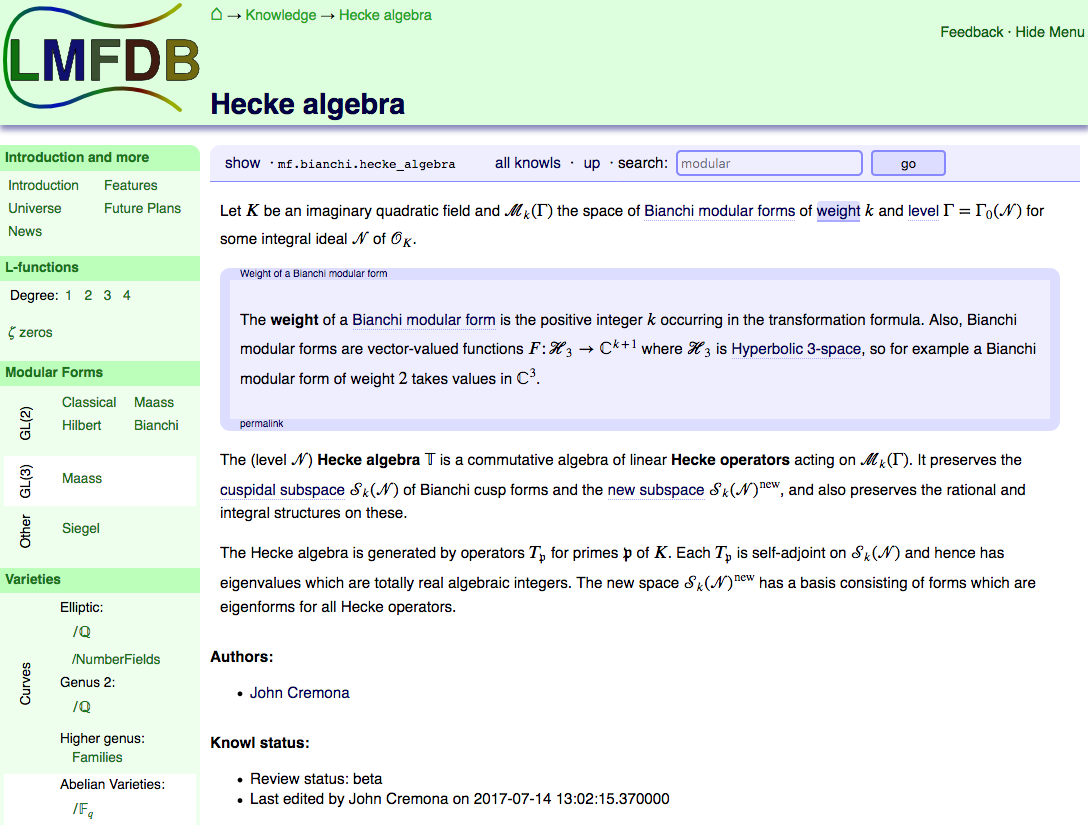
\includegraphics[width=14cm]{knowl}
  \caption{Knolws in the \LMFDB User Interface}\label{fig:knowl}
\end{figure}

\subsection{Alignments}\label{sec:integrating:alignments}

Finally we have to curate the \textbf{alignments} between the system dialects and the MitM ontology. 

To make the systems interoperable and translate objects and expressions, it is crucial to inform the system which symbols in the 
respective system API theories represent the same mathematical concepts. Then translation (as a first approximation) reduces to simply substituting symbols in an expression (see example below).\medskip

However, even when $A$ and $B$ deal with the ``same mathematical objects'', these may be constructed and represented differently, e.g., symbols can differ in name,
argument order/number, types, etc.
A major difficulty for system interoperability is correctly handling these subtle differences.
To formalize the details of this relation, \cite{MueGauKal:cacfms17} introduced \OMMT \textbf{alignments}.
Technically, these are pairs of \OMMT symbol identifiers decorated by a set of key-value pairs.
The alignments of $a$-symbols with the MitM ontology determine which $A$-objects correspond to MitM-objects.

The alignment of $a$-symbols to ontology symbols must be spelled out manually.
But this is usually straightforward and easy even for inexperienced users. For example, the following line aligns GAP's symbol \textsf{IsCyclic} (in the file \lstinline|lib/grp.gd|) with the corresponding symbol \textsf{cyclic} in the MitM ontology.
The key-value pairs are used to signify that this alignment is part of a group of alignments called ``VRE'' and can be used for translations in both directions.

\begin{lstlisting}
gap:/lib?grp?IsCyclic  mitm:/smglom/algebra?group?cylic
    direction="both" type="VRE"
\end{lstlisting}

Thus we can reduce the problem of interfacing $n$ systems to
\begin{inparaenum}[\em i\rm)]
\item curating the MitM ontology for the joint mathematical domain,
\item generating $n$ theory graphs for the system dialects,
\item maintaining $n$ collections of alignments with the MitM ontology.
\end{inparaenum}\medskip

Of course, in practice things are rarely as straight-forward, and subtle differences between implementations can require non-trivial translations. In those instances, we can simply formalize \emph{both} variants as separate symbols in the MitM ontology and move the translation process into the context of the latter, where we have \MMT \textbf{views} and other theory morphisms available.

The symbols in the system APIs can thus be aligned to the MitM formalization best suited for the specific implementation, and a conversion between two different variations (once modelled as a theory morphism) is available generically and for any pair of systems that diverge in their implementation the same way.
\medskip

For an example, consider again the dihedral group $D_4$ in \Sage (see Listings \ref{lst:sagedihedral:om} and \ref{lst:sagedihedral:xml}). We can align the relevant symbol 
\begin{lstlisting}
sage:?sage.groups.perm_gps.permgroup_named?DihedralGroup
\end{lstlisting}
with an abstract representation of dihedral groups in the MitM ontology (say, for instance \lstinline|mitm:?group?dihedralGroup|).
The \MMT system, when translating from \Sage to e.g. \GAP, then knows to replace the sage-specific symbol \lstinline|?DihedralGroup| by its system neutral equivalent in MitM, and the complex expression \lstinline+make_integer(4)+ by the plain OpenMath integer 4.
To translate the resulting statement in MitM to \GAP, we only need to align \lstinline+mitm:?Groups?dihedralGroup+ with the constructor for dihedral groups in \GAP, namely \lstinline+gap:/grp?basic?DihedralGroupCons+.

However, as mentioned in Section \ref{sec:intro} (Footnote 1), the implementations of dihedral groups in \Sage and \GAP differ with respect to their arguments -- the group labelled $D_4$ in \Sage is called $D_8$ in \GAP. So instead, we implement two different symbols in MitM, namely \lstinline|mitm:?group?dihedralGroupSmall| and \lstinline|mitm:?group?dihedralGroupLarge|, and align the \Sage symbol with the former and the \GAP symbol with the latter. Furthermore, we implement a view \lstinline|DihedralSmallToLarge: ?group->?group| in MitM, that maps $\lstinline|dihedralGroupSmall|(n)$ to $\lstinline|dihedralGroupLarge|(2n)$.


Translating to \GAP is then merely a matter of substituting the symbols in the OpenMath expression and applying the view (\GAP already uses OpenMath integers for remote procedure calls via \SCSCP) to reconstruct the original \Sage object in \GAP. Since there is exactly one path (vie alignments, includes or views) from the \Sage-expression to the corresponding \GAP-expression, this translation can be unambiguously found automatically (see \cite{MRLR:alignments:17}).

These alignments can be represented as in \ommt: 
\begin{lstlisting}[label=lst:dhalignments,caption=Alignments for Dihedral Groups]
sage:?sage.groups.perm_gps.permgroup_named?DihedralGroup
	mitm:?group?dihedralGroupSmall 
	direction="both" type="VRE"
gap:/grp?basic?DihedralGroupCons							
	mitm:?group?dihedralGroupLarge 
	direction="both" type="VRE"
\end{lstlisting}\medskip

They yield the stepwise translation given in Figure \ref{fig:sagetogap}

\begin{figure}
\lstset{basicstyle=\scriptsize\sf,aboveskip=-1.7ex,belowskip=-2.5ex}
\begin{tabular}{|lp{0.6\textwidth}|}\hline
  \Sage & \lstinline|DihedralGroup(4)| \\\hline
  OM (\Sage) &
\begin{lstlisting}
<OMA cdbase="http://python.org">
  <OMS name="DihedralGroup" 
  	cd="sage.groups.perm_gps.permgroup_named"/>
  <OMA>
    <OMS name="make_integer" cd="sage.rings.integer"/>
    <OMI>4</OMI>
  </OMA>
</OMA>
\end{lstlisting}\\\hline
OM (MitM) &
\begin{lstlisting}
<OMA cdbase='http://mathhub.info/MitM/Core'>
  <OMS name='dihedralGroupSmall' cd='group'/>
  <OMI>4</OMI>
</OMA>
\end{lstlisting} \\
OM (MitM, after applying view) &
\begin{lstlisting}
<OMA cdbase='http://mathhub.info/MitM/Core'>
  <OMS name='dihedralGroupLarge' cd='group'/>
  <OMI>8</OMI>
</OMA>
\end{lstlisting}
\\\hline
  OM (\GAP) &
\begin{lstlisting}
<OMA cdbase='http://www.gap-system.org/grp'>
  <OMS name='DihedralGroupCons' cd='basic'/>
  <OMI>8</OMI>
</OMA>
\end{lstlisting}
  \\\hline
	\GAP & \lstinline|DihedralGroupCons(8)|\\\hline
\end{tabular}
\caption{Stepwise Translation of Dihedral Group $D_4$ from \Sage to \GAP using the alignments from Listing~\ref{lst:dhalignments}}\label{fig:sagetogap}
\end{figure}

Alignments form an independent part of the MitM interoperability infrastructure.
Incidentally, they obey a separate development schedule: the MitM ontology is developed by the community as a whole as the understanding of a mathematical domain changes.
The system dialects are released together with the systems according to their respective development cycle.
The alignments bridge between them and have to mediate these cycles.

These alignments are currently produced and curated using the approach, repository, and syntax described in~\cite{MueGauKal:cacfms17,MueRoYuRa:abtafs17}.
In the future, we will also consider automatically extracting alignments from the existing ad-hoc \Sage-to-$X$ translations.
These are (mainly) given as \Sage code annotations that relate \Sage operations and constructors with those of system $X$.

Figure~\ref{fig:cgtontology} shows some example alignments between symbols in the GAP content dictionary and the MitM ontology.




%%, but from some of the initial alignments and the \GAP API theories we will be able to infer more alignments automatically.
%%For example, the filter \texttt{GAP:IsGroup} is aligned with
%%\texttt{mitm:Group}, and the filter \texttt{GAP:IsPermGroup} is aligned with
%%\texttt{mitm:Subgroup SymmetricGroup [1..n]}.
%
%We formalized the theory of symmetric groups of a set in the MitM ontology.
%In \GAP, permutation groups are represented as subgroups (with finite support) of the symmetric group of $\mathbb{N}+$, and often one concretely has an isomorphism between the group one is interested in and a subgroup of $S_{\mathbb{N}+}$, for example via a group action.

%\texttt{SylowSubgroup}s are more difficult: They are special groups in their own right, namely groups whose size is a prime-power, but we also want them to be identified with a certain subgroup of the group we are working with.
%\ednote{MP: While I believe this to be an excellent additional example for \OMMT formalisation, this could be going too far for this paper}

%\ednote{MK@MK: still to write: the alignment-based priorization and suggestion mechanism. }


%%% Local Variables:
%%% mode: latex
%%% TeX-master: "report"
%%% End:

%  LocalWords:  DehKohKon:iop16 emph serialization sec:mitm deserializes subsubsection MueGauKal:cacfms17 MueRoYuRa:abtafs17 defemph defemph texttt texttt texttt texttt compactenum serializes lst:sagedihedral papertype ednote subtyping Cremona:LMFDB16,lmfdb:on knowls fig:knowl knowl knowl Kohlhase:ulsmf08 pdflatex flexiformal centering includegraphics Knolws inparaenum medskip MueGauKal:cacfms17,MueRoYuRa:abtafs17
%  LocalWords:  analyze itemize Deserialization serialized lstlisting pg_unreduce mathbb
%  LocalWords:  unpickle_global unreduce pg_DihedralGroup serializer py-openmath:on
%  LocalWords:  lstinline optimizations factorization serialize deserialized deserializer
%  LocalWords:  fig:cgtontology GroupHomset serializing analyzed py-scscp:on mitm:Group
%  LocalWords:  mitm:Subgroup SylowSubgroup newpart priorization summarize compactitem
%  LocalWords:  formalized
